% TODO

\begin{figure}[h]
    \newcommand{\tempStmtA}{\sSkip
                    ~|~ \sDeclare {$T$} {$x$}
                    ~|~ \sFieldAssign {$x$} {$f$} {$y$} 
                    ~|~ \sVarAssign {$x$} {$e$}
                    ~|~ \sAlloc {$x$} {$C$} 
                    ~|~ \sCall {$x$} {$y$} {$m$} {$z$}}
\newcommand{\tempStmtB}{~~~ ~|~ \sReturn {$x$}  
                            ~|~ \sAssert {$\phi$} 
                            ~|~ \sRelease {$\phi$} 
                            ~|~ \sHold {$\phi$} {$s$}
                            ~|~ \sSeq {$s_1$} {$s_2$}}
\newcommand{\tempFrm}{  \phiTrue 
                    ~|~ \phiEq {$e$} {$e$} 
                    ~|~ \phiNeq {$e$} {$e$}
                    ~|~ \phiAcc {$e$} {$f$}
                    ~|~ \phiCons {$\phi$} {$\phi$}}
\newcommand{\tempExpr}{ \ev{$v$}
                    ~|~ \ex{$x$}
                    ~|~ \edot{$e$}{$f$}}

\begin{align*}
	program  & \in \setProgram    &  & ::= \ttt{$\overline{cls}$~$\overline{s}$}                         \\
	cls      & \in \setClass      &  & ::= \class {$C$} {$\overline{field}$} {$\overline{method}$}       \\
	field    & \in \setField      &  & ::= \field {$T$} {$f$}                                            \\
	method   & \in \setMethod     &  & ::= \method {$T$} {$m$} {$T$} {$x$} {$contract$} {$\overline{s}$} \\
	contract & \in \setContract   &  & ::= \ttt{requires $\phi$;~ensures $\phi$;}                        \\
	T        & \in \setType       &  & ::= \Tint ~|~ C                                                   \\
	s        & \in \setStmt       &  & ::= \tempStmtA                                                    \\
	         &                    &  & \tempStmtB                                                        \\
	\phi     & \in \setFormula    &  & ::= \tempFrm                                                      \\
	e        & \in \setExpr       &  & ::= \tempExpr                                                     \\
	x, y, z  & \in \setVar        &  & ::= \ethis ~|~ \eresult ~|~ name                                  \\
	v        & \in \setVal        &  & ::= o ~|~ n ~|~ \enull                                            \\
	o        & \in \setObj        &  &  \\
	n        & \in \mathbb{Z}     &  &  \\
	C        & \in \setClassName  &  & ::= name                                                          \\
	f        & \in \setFieldName  &  & ::= name                                                          \\
	m        & \in \setMethodName &  & ::= name
\end{align*} 
    \caption{\svlidf: Syntax}
    \label{fig:idf-syntax}
\end{figure}

%% parser rassoc, skip
We pose $\phiFalse \defeq \phiNeq{\enull}{\enull}$.
We define $\ttt{;}$ to be right-associative and assume that parsing a sequence of statements (e.g. method body) operates analogously, obviating the need for parenthesis.
Furthermore we assume that the parser terminates every sequence with $\sSkip$.
\begin{exmp}~
    \begin{lstlisting}
    ...
    {
        $s_1$;
        $s_2$;
        $s_3$;
    }
    \end{lstlisting}
    is parsed as
    
    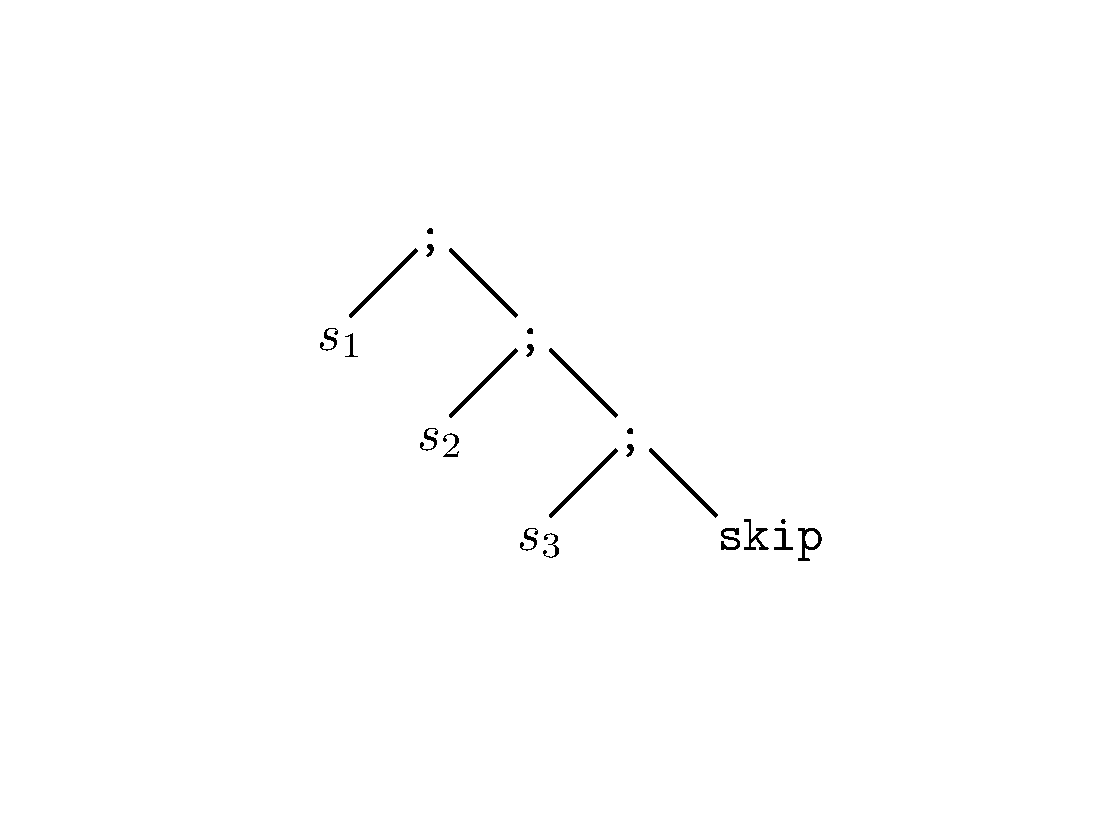
\includegraphics[trim={3cm 3cm 3cm 3cm}, clip, width=6cm]{graphics/rightAssocSkip}
\end{exmp}
These assumptions highly simplify reasoning about statements.

%% helper methods
We define the following helper methods:
\begin{figure}[h]
    We define the following helper methods:

\begin{description}
    \item[Extraction]
    To extract elements from a given program $p \in \setProgram$ we define the following functions:
    \begin{align*}
    	 & \fieldType : \setClassName \times \setFieldName \rightharpoonup \setType                & ~ \\
    	 & \fieldType(C, f) = \text{type of field $f$ in class $C$ in $p$}                         &  \\
    	 & ~                                                                                       &  \\
    	 & \predicate{fields$_p$} : \setClassName \rightharpoonup \PP^{\setField}                  &  \\
    	 & \fields{C} = \text{field declarations of class $C$ in $p$}                              &  \\
    	 & ~                                                                                       &  \\
    	 & \predicate{method$_p$} : \setClassName \times \setMethodName \rightharpoonup \setMethod &  \\
    	 & \mmethod{C, m} = \text{declaration of method $m$ in class $C$ in $p$}                   &  \\
    	 & ~                                                                                       &  \\
    	 & \predicate{mpre$_p$} : \setClassName \times \setMethodName \rightharpoonup \setFormula  &  \\
    	 & \mpre{C, m} = \text{precondition of method $m$ in class $C$ in $p$}                    &  \\
    	 & ~                                                                                       &  \\
    	 & \predicate{mpost$_p$} : \setClassName \times \setMethodName \rightharpoonup \setFormula &  \\
    	 & \mpost{C, m} = \text{postcondition of method $m$ in class $C$ in $p$}                   &
    \end{align*}
    
    \item[Free Variables]~\\
    The semantics of \svlidf will sometimes reason about the free variables of expressions or formulas.
    
    Let $\FV : (\setExpr \cup \setFormula) \rightarrow \PP^{\setVar}$ be defined as
    \begin{alignat*}{3}
    	  & \FV(v)                            &  & = \emptyset                    & ~ \\
    	  & \FV(x)                            &  & = \{ x \}                      &  \\
    	  & \FV(\edot{$e$}{$f$})              &  & = \FV(e)                       &  \\
    	~ &  \\
    	  & \FV(\phiTrue)                     &  & = \emptyset                    &  \\
    	  & \FV(\phiEq{$e_1$}{$e_2$})         &  & = \FV(e_1) \cup \FV(e_2)       &  \\
    	  & \FV(\phiNeq{$e_1$}{$e_2$})        &  & = \FV(e_1) \cup \FV(e_2)       &  \\
    	  & \FV(\phiAcc{$e$}{$f$})            &  & = \FV(e)                       &  \\
    	  & \FV(\phiCons{$\phi_1$}{$\phi_1$}) &  & = \FV(\phi_1) \cup \FV(\phi_2) &
    \end{alignat*}
    
    \item[Default Value of Type]~\\
    \svlidf assigns default values to declared variables.
    
    Let $\predicate{defaultValue} : \setType \rightarrow \setVal$ be defined as
    \begin{alignat*}{3}
    	 & \defaultValue{\Tint} &  & = 0      & ~ \\
    	 & \defaultValue{$C$}   &  & = \enull &
    \end{alignat*}
    
    \item[Required Access]~\\
    Expressions mentioning fields are heap-dependent and thus require access.
    To enable treating expressions in a uniform fashion, we define a pseudo accessibility-predicate which is also defined for expressions that do not mention fields.
    
    Let $\predicate{acc} : \setExpr \rightarrow \setFormula$ be defined as
    \begin{alignat*}{3}
    	 & \accFor{v}               &  & = \phiTrue          & ~ \\
    	 & \accFor{x}               &  & = \phiTrue          & ~ \\
    	 & \accFor{\edot{$e$}{$f$}} &  & = \phiAcc{$e$}{$f$} &
    \end{alignat*}
    
    \item[Preventing Writes]
    Under rare circumstances, overwriting a certain variable is not allowed in \svlidf.
    To reliably check which variables are written to by a statement, we define the following function.
    
    Let $\mods : \setStmt \rightarrow \PP^{\setVar}$ be defined as
    \begin{alignat*}{3}
    	 & \mods({\sVarAssign {${x}$} {${e}$}})            & ~ & = \{~ x ~\}                       & ~ \\
    	 & \mods({\sAlloc {${x}$} {${C}$}})                & ~ & = \{~ x ~\}                       & ~ \\
    	 & \mods({\sCall {${x}$} {${y}$} {${m}$} {${z}$}}) & ~ & = \{~ x ~\}                       & ~ \\
    	 & \mods({\sReturn {${x}$}})                       & ~ & = \{~ \eresult ~\}                & ~ \\
    	 & \mods({\sDeclare {${T}$} {${x}$}})              & ~ & = \{~ x ~\}                       & ~ \\
    	 & \mods({\sHold {${p}$} {${s}$}})                 & ~ & = \mods(s)                        & ~ \\
    	 & \mods({\sSeq{$s_1$}{$s_2$}})                    & ~ & = \mods(s_1) \cup \mods(s_2)      & ~ \\
    	 & \mods(s)                                        & ~ & = \emptyset \textit{~~~otherwise} & ~
    \end{alignat*}
    %% Inductive writesTo
\begin{mathpar}
\inferrule* [Right=wtVarAssign]
{
    ~
}
{
    \writesTo({x}, {\sVarAssign {${x}$} {${e}$}})
}
\end{mathpar}

\begin{mathpar}
\inferrule* [Right=wtAlloc]
{
    ~
}
{
    \writesTo({x}, {\sAlloc {${x}$} {${C}$}})
}
\end{mathpar}

\begin{mathpar}
\inferrule* [Right=wtCall]
{
    ~
}
{
    \writesTo({x}, {\sCall {${x}$} {${y}$} {${m}$} {${z}$}})
}
\end{mathpar}

\begin{mathpar}
\inferrule* [Right=wtReturn]
{
    ~
}
{
    \writesTo({\eresult}, {\sReturn {${x}$}})
}
\end{mathpar}

\begin{mathpar}
\inferrule* [Right=wtDeclare]
{
    ~
}
{
    \writesTo({x}, {\sDeclare {${T}$} {${x}$}})
}
\end{mathpar}

\begin{mathpar}
\inferrule* [Right=wtHold]
{
    {s} \in {ss} \\
    \writesTo({x}, {s})
}
{
    \writesTo({x}, {\sHold {${p}$} {${ss}$}})
}
\end{mathpar}


\end{description}
    \caption{\svlidf: Helper Methods}
    \label{fig:idf-helpers}
\end{figure}


%% other stuff
For future reference, we give further (non-syntactic) definitions:
\begin{figure}[h]
    \begin{align*}
    A_s    & \in \setSFootprint &  & =~~ \PP^{\setExpr \times \setFieldName}                                                    \\
    A_d    & \in \setDFootprint &  & =~~ \PP^{\setLoc \times \setFieldName}                                                     \\
    \Gamma & \in \setTypeEnv    &  & =~~ \setVar \rightharpoonup \setType                                                       \\
    \rho   & \in \setVarEnv     &  & =~~ \setVar \rightharpoonup \setVal                                                        \\
    E      & \in \setStackEntry &  & =~~ \setVarEnv \times \setDFootprint \times \setStmt                                       \\
    S      & \in \setStack      &  & ::= E \cdot S ~|~ \nil                                                                     \\
    H      & \in \setHeap       &  & =~~ \setLoc \rightharpoonup (\setClassName \times (\setFieldName \rightharpoonup \setVal))
    \end{align*}
    \caption{\svlidf: Further Definitions}
\end{figure}



% Programs consist of classes and a main method, represented directly as the list of its instructions.
% TODO: introduce all the extraction predicates/functions!
